\chapter{CMS}
Before we start analyzing the strcture and the implementation details of a new
generation CMS it is worth giving a definition to a Content Management System.
Apart form that in the current chapter we will discuss the types of CMS's that
exist nowadays. Finally, we will concentrate on the Magnolia CMS which is the
target system of the current paper: the high-level structure and main features
of it will be highlighted.

\section{Definition of a CMS}
A \emph{Content Management System or CMS} could be defined as a server-side
software that is designed to simplify the creation and maintenance of websites.
These systems manage online content, generate Web pages, and allow users to
upload and change content without requiring technical expertise. The foundation
of almost every CMS is a data storage of a varying type like, for instance, a
database or a repository which stores the content allowing it to be reused,
repurposed or published on demand.

Another crucial part of every CMS is the administration interface. It interacts
with the storage and provides users with various tools starting from
input/upload of content to complex editors and asset managers.
Typically this administration interface is implemented in the form of a web
application. The biggest advantage of this approach is that the actual content
resides within easy reach from any location having internet access.

However, acting just as a data storage management tool would not make any CMS a
valuable or highly useful product. The main purpose of a CMS is to build the Web
Site around the content. This involves several fundamental concepts:
\begin{itemize}
	\item Template mechanism. Normally the system is shipped with the  templating
	framework. This framework is a higher level abstraction on top the ordinary
	programming language and allows for the building of complex pages with less
	effort.
	Applying the specific template to the raw content from the repository is a
	concept idea of making web-pages with CMS's.
	Different systems offer different levels of flexibility allowing to partially or
	completely change the templates, or to create new templates and themes.

	\item Automation of page generation. A CMS often provides the engine that would
	generate the typical pages on demand or request. A good example would be a blog
	post or a forum thread.
	
    \item Navigation handling. A CMS provides an easy and almost automated way to
    set references between parts of the web site and to manage them on the high
    level.
	
	\item Basic Search Engine Optimiation (SEO). (TODO: Add how)
\end{itemize}


\section{Types of CMS} 
There are numerous CMS's existing nowadays. As it was mentioned
before a CMS can be developed with different programming languages, e.g.
\emph{Plone CMS} is written in Python, \emph{Drupal} and \emph{Joomla} are
written in PHP and \emph{OpenCMS} is written in Java.

Each CMS is trying to occupy some certain niche and to solve problems of
different scope. There are some systems that are highly powerful only for some
specific use cases, for instance \emph{Wordpress} is usually used for developing
blogs and \emph{Liferay} is a platform for the portals.

There are both proprietary (like \emph{Alphresco}) and open source CMS's (like \emph{MODx}).
The licences and usage policies also vary.

\section{Importance of CMS's in the Modern World Wide Web}
Content Management Systems play a significant role in modern web development.
There are several strong reasons for that.

First of all, as it was mentioned before, adopting a CMS in the project provides
a solution for the most common problems a website developer faces. This can
dramatically increase the development speed allowing the team to concentrate on
business logic and higher level problems. In addition if the project is built on
top of a popular CMS - the chances of finding a relevant expert are a lot higher
than in the case of a completely custom made project.

What is more, a CMS offers a solid foundation which makes it easier to build
scalable, robust and responsive websites: many CMS's provide architecture for
clustering, while a time proven storage API ensures the safety of the data.

Another important advantage of Content Management Systems is that people without
advanced technical skills can use them.
A CMS with a powerful administration interface usually does not require
programming experience (neither client side like JavaScript/HTML/CSS, nor server
side like PHP or Java) to edit or add a page, upload data or change user
permissions. As a consequence the support of CMS-based projects is a lot
simpler. After shipping the product the development team can usually educate the
customer on how to use the admin tool and at least partially delegate the
maintenance chores to them.

There is no surprise in that almost one third of all websites in the WWW use a
CMS. The tendency depicted in Figure 1 shows that this amount is growing
\cite{cms_growth}.
\begin{figure}[H]
	\centering
	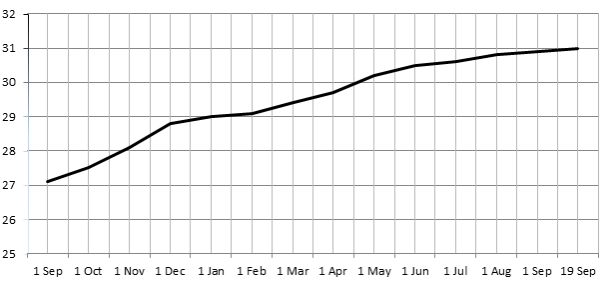
\includegraphics[width=\textwidth]{cms_usage_growth.png}
	\caption{CMS usage growth trend}
	\label{fig:cms_usage_growth}
\end{figure}

\section{Drawbacks of Using a CMS}
Obviously a CMS is not a silver bullet for all the problems. In spite of
reducing the project costs, speeding up the development process and allowing
users to avoid any kind of programming, usage of a CMS has several negative
aspects that should be kept in mind.

Sometimes non-technical companies adopt a CMS only in order to avoid learning
any programming language. This might not prove itself on the long run because
sooner or later a certain level of programming proficiency will be required.
This is dictated by the limitations of the templating mechanism which usually
requie designer skills to be properly surpassed.

Another case is the limitations of the administration interface: the specific
projects' authors might for example requires a special search tool or they need
to be able to observe the structure of their website in a form that is different
from those offered by the CMS they use. Finding a workaround would require some
backend programming experience or outsourced professional's help.
The complexity of the solution also depends a lot on the CMS administration
tools' ability to be extended. A good proof of such drawback could be the
results of the survey conducted by the Webcredible company several years ago.
According to it the practical factors such as the range of the offered features
(22 per cent), convenience (21 per cent) and ability to customize the
functionality were key when choosing a CMS. According to the Webcredible
authorities the results showed a high amount of respondents who were frustrated
with the poor user experience with the chosen CMS. The main reason for
dissatisfaction was the lack of attention to the end user needs resulting into a
product that is oriented on the technical people. Inability to extend the
system, add and replace modules on demand was also mentioned as a reason against
some systems.

\section{Magnolia CMS}
The Magnolia CMS is one of the leading enterprise-oriented CMS's. It is
implemented using the Java programming language by Magnolia ltd., a company
located in the city of Basel, Switzerland. Magnolia is based on Jackrabbit
(JSR-170/JCR reference implementation) and focuses on medium to large
enterprises[2].

\subsection{Features of Magnolia CMS}
As long as Magnolia CMS is the main subject of this paper let us observe the
main features and advantages of the system, the position that it holds in the CMS world.

\subsubsection{Modular Structure}
The architecture of Magnolia CMS can be described as loosely coupled and
flexible. The system consists entirely out of modules.  A module is an
independent component that performs a particular task or packages content and
functionality[2].
A good module example could be the AdminCentral (an admin interface of the CMS)
or the Blossom (Spring Framework Integration Module). A module can be used to
encapsulate a specific solution or a feature implementation e.g. a forum module
which is used for building discussion threads. It is also possible to make asset
bundles that can contain images or documents.
In some cases it becomes convenient to package an entire website with all the
content and templates to for example increase the deployment speed.

\subsubsection{Templating}
All Web pages created with the Magnolia CMS are based on templates. Templates
ensure that page structure and presentation remain the same while the content
varies from one page to another. For example, an event template helps you
generate event pages that look and feel the same while each of them displays a
different unique event.

The system generates pages by merging a template with corresponding content from
the repository. The position and inclusion of each paragraph on the page is
defined by the page template. In many instances, the page template will allow
authors to choose from a number of different paragraph types in a single content
area[2].

\subsubsection{Scalability}

The Magnolia CMS is distributed as two web-applications, one acting as the
authoring instance and the other as the public environment (see \ref{fig:scalability}). This allows for
better security, having one application inside your firewall and one outside. It
also enables clustering configurations.
\begin{itemize}
	\item Author instance is where all authors work. It typically resides in a
	secure location such as behind a corporate firewall, inaccessible from the
	Internet. The author instance publishes content to public instances.
	\item Public instance receives the public content and exposes it to visitors on
	the Web. It resides in a public, reachable location. It is possible to have more
	than one public instance serving the same or different content.
\end{itemize}
\begin{figure}[H]
	\centering
	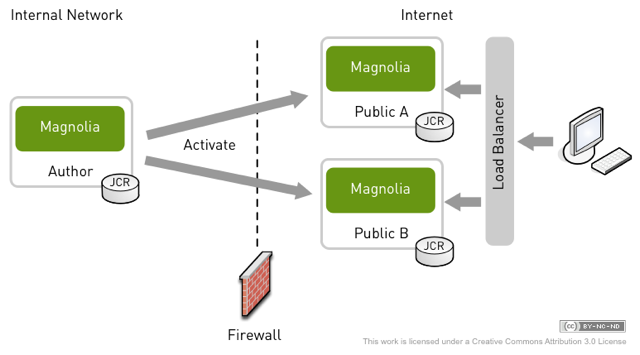
\includegraphics[width=\textwidth]{scalability.png}
	\caption{Magnolia CMS scaling strategy}
	\label{fig:scalability}
\end{figure}

\subsubsection{JSR-170}
Java Content Repository (JCR) is the core underlying technology for storing and
managing data in Magnolia CMS. JCR is a standard programming interface for
communication with content repositories. JCR was first established in Java
Specification Request 170 (JSR-170). Current JCR version 2.0 was finalized in
JSR-283. JCR is able to handle both structured and unstructured content
specified within hierarchical storage. Magnolia CMS uses Apache Jackrabbit
reference implementation of JCR and within the scope of current paper adheres to
the Java Content Repository standard.

\paragraph{Content Repository} stands for a high-level data management system
allowing for various operations to be performed over the stored content. These
are the most essential features of a Content Repository:

\begin{itemize}
  \item Aforementioned ability to store either structured content (e.g. Extensible Mark-up Language (XML)
  files, page templates etc) or unstructured (e.g. Binary Large OBjects (BLOB)).
  \item Referential integrity: support for primary and foreign keys and handling
  the violation of them.
  \item Querying data. The typical language to acces content repository is XML Path Language (XPath) \cite{xpath} 
  XPath. However, Structured Query Language (SQL) dialects usually can also be used.
\end{itemize}

A Magnolia CMS instance works with a single repository (called
\texttt{magnolia}). Semantic separation between datasets is provided with
\emph{workspaces}. Workspace is a tree-like structures with a single root.
The leaves of such a tree are called \emph{properties}. \emph{Properties} carry the all the
actual content of the repository.

From the perspective of this thesis, the most important workspaces of the Magnolia CMS are:
\begin{itemize}
  \item \emph{website} Stores the pages, paragraphs and most of the content  for the websites.
  \item \emph{config} The configuration settings.
  \item \emph{DAM} Workspace for Dynamic Asset Management.
  \item \emph{users} Stores all the types of user accounts (administrative, system public etc).
\end{itemize}

 We will especially concentrate on the \emph{config} workspace as configuration
 will play a significant role in the
foundation for the flexible user interface (see Chapter \ref{architecture}). We will
also touch the \emph{DAM workspace} when we will discuss the Asset Management in
the Chapter \ref{implementation}.


\subsubsection{Admin Central}
The Admin Central is the core module of Magnolia which gives the chrome for
administration and website management. Provides tools for editing publishing
and verifying the pages.\cite{magnolia_shell}

\subsubsection{Position in the CMS World}
Due to a flexible and highly customizable architecture that follows the best
Java patterns and practices, Magnolia CMS has managed to attract many serious
enterprises. Such companies as Allianz, Foxtel, Sony, Thomas Cook, Michelin,
U.S. Navy, Rewe, MBC Group, EADS, ING Bank, Atlassian and Migros and many others
in more than 100 countries \cite{magnolia_customers}.
\pagebreak